\documentclass[a4paper,11pt,twocolumn,twoside]{article}
\usepackage{fullpage}
\usepackage{graphicx}
\usepackage{pgfplots}
\usepackage{pgfplotstable}
\usepackage{filecontents}
\usepackage{booktabs}
\usepackage{tabularx}
\usepackage{tikz}
\usepackage{listings}
\usepackage{authblk}

\usetikzlibrary{patterns,shapes,positioning,calc}

\lstset{language=C, basicstyle=\ttfamily, columns=flexible}

\pgfplotsset{compat=1.8}

\author{Lars Kirkholt Melhus}
\author{Rune Erlend Jensen}
\affil{Norwegian University of Science and Technology}
\title{Sources of Measurement Bias on Modern CPUs}
\date{} % This is a timeless piece

\begin{document}

\twocolumn[
  \begin{@twocolumnfalse}
    \maketitle
    \begin{abstract}
    Seemingly innocuous properties of the execution context, such as the contents of system environment variables, or variations in link ordering, can impact the performance of computer programs. 
    Variations in external properties like these can bias programs towards certain configurations. 
    These effects have been shown to be a significant issue in performance analysis, but unpredictable and difficult to deal with.

    Abstract This paper focuses on the underlying reasons for bias effects that can be experienced for example by changing environment variables, or using different link orders. 
    Through experimentation and careful measurements using performance counters, we identify several potential sources of bias on the 4th generation Intel Core i7 architecture Haswell. 
    Limitations imposed by the Loop Stream Detector is revealed, along with effects from 4K address aliasing. We show that bias is in fact not completely unpredictable, and discuss measures for avoiding it.
    \end{abstract}
    \bigskip
        
  \end{@twocolumnfalse}
]


\section{Introduction}
Optimizing for performance is an important topic in computer science, and high performance computing (HPC) in particular. 
A great amount of research and effort is put into designing better algorithms and compiler optimizations, in order to produce an “optimal” executable. 
However, performance of computer programs is not just a function of the collection of machine instructions executed. 
Various external properties, such as the operating system and user environment, can have have an impact on how fast programs execute. 
Characteristics of the operating system can decide things like the placement of code and data in memory, which in turn interacts with various hardware mechanisms. 
Corner cases in hardware introduces potential performance cliffs; If for example a memory access happens to cross a page boundary, the cost of an additional TLB miss can be significant. 
The set of conditions under which a program executes is called the execution context, which includes virtual memory layout in particular. 
Variations within contexts can lead to programs being biased towards certain configurations. 
Measuring performance of the same program on two machines with identical hardware can sometimes yield very different results, an effect known as measurement bias.

Previous work has studied parameters such as the size of Unix environment variables and program link order. 
Both are found to potentially have a significant effect on performance, even in standardized benchmarks. 
Unfortunately, the effects also appear to be unpredictable, and therefore difficult to deal with. 
This poses a problem for researchers and performance analysts, who will need to account for effects of measurement bias with more rigorous methodologies and statistical methods.

Both the size of environment variables and link ordering ultimately has an effect on memory layout of running processes. 
We will not look at things like cache efficiency, which often can be the reason for bad performance under certain memory contexts. 
Instead, we look at effects from less known optimizations in the out-of-order execution engine and instructions fetch pipeline. 
Because bias effects are intrinsically connected to various hardware features, this paper is focued on the Intel® Core™ i7 “Haswell” architecture specifically. 
However, the bias sources we present has also been shown to behave similarly on previous Intel architectures as well.
With a better understanding of intricate properties of the CPU, we show how one is able to not only predict, but also explicitly optimize for beneficial memory layouts. 

In the paper appropriately named “Producing Wrong Data Without Doing Anything Obviously Wrong” by T. Mytkowicz et al. \cite{Mytkowicz:2009:WrongData}, the authors show how simple changes to the execution environment can have an impact on performance. 
One of their examples is a program where performance varies significantly with changes to the environment variables. 
Unix environment variables contain various information about the system, such as the name of the currently logged in user, home- and current directory path.
This means that the length of your name -- by extension you user login -- could in principle be the tipping point between good and bad performance.

Previous work focuses mostly on how to mitigate effects of bias, and avoid drawing the wrong conclusions based on misleading measurements \cite{Mytkowicz:2008:Easy, Mytkowicz:2009:WrongData}.
The goal of this paper is to show not only that bias exists, but also \emph{why} it occurs. 

With more accurate models of how bias occur, we will not only be able to actively avoid in performance, but in some cases also gain a real speedup on average.

Modern microprocessors are extremely complex in design and functionality. 
Some features of recent Intel processors includes several layers of cache to camouflage slow memory, multiple prefetchers, speculative out-of-order execution and branch prediction, just to name a few.
Hardware features and optimizations interact with memory layout of program code and data in various ways.
We will unveil characteristics about two different architectural features in recent Intel CPUs, and show how they can bias performance towards certain memory contexts. 

First we will look at an aliasing effect between memory addresses of loads and stores, causing false dependencies in the out-of-order execution pipeline. 
This effect can be triggered for example by changing stack position, and can explain bias from altering environment variables. 
Secondly, we will look at the Loop Stream Detector, which in previous work on measurement bias has been suggested as a possible explanation.
We therefore choose to study this particular optimization in detail, and show how measurement bias can occur from changing link order.


\section{Methodology}
When studying bias effects, carefully controlling all relevant properties of the environment is crucial. 
Previous work on measurement bias and observer effect describes a set of best practices for how the measurement infrastructure should be configured \cite{Mytkowicz:2009:WrongData, Mytkowicz:2008:OE&MB}. 
\begin{itemize}
  \item Address space layout randomization (ASLR) is disabled
  \item Hyper-threading is disabled
  \item System load is kept at a minimum
  \item Automatic CPU frequency scaling is disabled
\end{itemize}
Our hardware configuration consists of an Intel® Core™ i7-4770K @ 3.50 GHz and 32 GB DDR3 @ 1600 MHz, running a 64-bit installation of Ubuntu 13.10. GCC version 4.8.1 is used as compiler toolchain.

We use perf to acquire statistics and measurements.
Perf is a utility to interface with hardware performance counters, and available as part of the Linux kernel.
Measurements are aggregated over several runs to collect all of the about 200 performance counters provided on our architecture [Intel:2013:Volume3B]. 
Unless otherwise specified, a minimal environment is used for all benchmarks. 
To measure statistics with n bytes added to the environment, a dummy variable is set to \(0^{n}\) (repeated zero characters n times).

Cache conflicts can in many cases be a potential explanation for bias effects observed by changing memory layout.
Although cache is often a likely explanation of performance variations, bias caused by cache issues is well understood and \emph{not} the focus of this paper.
Cache related metrics are monitored in order to rule out cache as the underlying cause of bias. 
The hit rates of micro-ops for each level of cache can be monitored by performance counters \cite{Intel:2012:OptimizationManual}.


\section{4K Address Aliasing}
An event known as “4K aliasing” can occur when the addresses of a store instruction followed by a load instruction differ by a multiple of 4 KiB.
On recent Intel architectures, only the last 12 address bits are used to determine if operations refer to the same address \cite{Intel:2012:OptimizationManual}.
This is a heuristic employed by the CPU to enable out of order execution of memory access operations.
Independent pairs of loads and stores where the last address bits differ can then be reordered and issued out of order.
Doing only a partial compare, \emph{false} dependencies can be detected when the addresses are equal $\bmod 4096$, as in the following example: 
\begin{lstlisting}[language={[x86masm]Assembler}]
mov %rax ($0x601010)
mov ($0x604010) %rbx
\end{lstlisting}
Situations like these causes the pipeline to stall and wait for the operations to finish in proper order.
The number of times this happens can be counted by the following performance counter:
\begin{description}
  \item{LD\_BLOCKS\_PARTIAL.ADDRESS\_ALIAS}\marginpar{\small{Evnt Mask \\ 0x07 0x01}} \hfill \\
  Counts the number of loads that have partial address match with preceding stores, causing the load to be reissued.
\end{description}
Performance implications of 4K aliasing is discussed to some extent in the optimization manual from Intel. 
There are even some concrete suggestions for how avoid aliasing cases to improve performance (Rule 8 and 9) \cite{Intel:2012:OptimizationManual}.
In the following sections, we look at how address aliasing can explain some instances of measurement bias.

\subsection{Bias from Environment Size}
Variations in performance with bias towards certain environment sizes has been observed by other authors.
Unless the program explicitly accesses environment variables, it is not the environment variables themselves that are important, but rather the effect their total size has on the alignment of stack. 
Figure \ref{fig:stack} shows the relative positions of some important sections of memory at run time, assuming a 64 bit process mapped to virtual memory. 

\pgfplotstableread{resources/stack-offset.dat}{\stackoffsettable}
\begin{figure*}[t]
  \caption{Bias from environment size}
  \begin{tikzpicture}
    \begin{axis}[
        width = \textwidth,
        height = 6cm,
        font = \small,
        xlabel=Bytes added to environment,
        domain = 0:8192,
        xtick = {0,1024,...,8192},
        xmin = 0,
        xmax = 8192,
        legend pos = outer north east,
        cycle list name = exotic
      ]
      %\draw [<->, line width=0.8, color=red] (axis cs:0,8e5) -- (axis cs:4096,8e5) ;
      \addplot[ycomb] table[x expr = \thisrowno{0}*16, y = cycles:u] \stackoffsettable ;
      %\addplot table[x expr = \thisrowno{0}*16, y = r0107:u ] \stackoffsettable ;
      \addlegendentry{cycles:u} ;
      \addlegendentry{r0107:u} ;
    \end{axis}
  \end{tikzpicture}
\end{figure*}

The stack is normally placed close to the upper address 0x7fff'ffffffff.\footnote{Modern processors do not actually use the full 64 bit space, only the low order 47 bits are used for addressing memory}
Environment variables and program arguments are allocated in the stack section, before the first call frame.
Changing environment variables will therefore offset the addresses of all stack allocated data.
There is still some level of stack alignment happening, independent of environment offsets. 
The compiler can enforce alignment to some number of zero bits.
As long as this number is less than 12, environment size can impact addresses of automatic variables $\bmod 4096$.

Text and data sections contain program code and static data respectively.
These regions are mapped towards the low en of the address spectrum, and the virtual addresses of variables allocated here will not change with environment size. 

Note that the initial position of stack will not depend on environment size this way when address randomization (ASLR) is enabled. (TODO: Does it offset from page boundary? That would be good, same alias behavior :)

\begin{figure}
  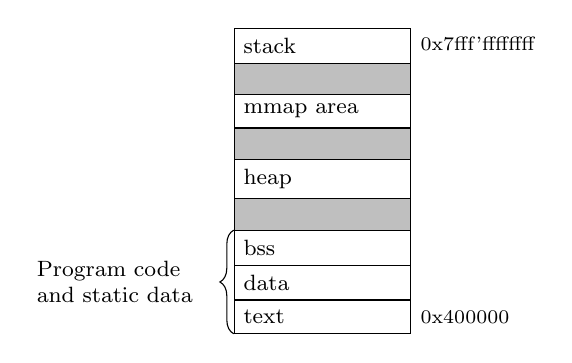
\begin{tikzpicture}[font=\footnotesize]

    % See page 453 in pgf manual
    \node [
      rectangle split, rectangle split parts=9, 
      rectangle split part fill={white, lightgray, white, lightgray, white, lightgray, white},
      draw, anchor=center, text width=2cm
    ] (m)  
      {
        \nodepart{one}
          stack
        \nodepart{three}
          mmap area
        \nodepart{five}
          heap
        \nodepart{seven}
          bss
        \nodepart{eight}
          data
        \nodepart{nine}
          text
      };

    \draw [decorate, decoration={brace, amplitude=5pt}] (m.south west) -- (m.six split west) 
      node [black, midway, xshift=-1.5cm, text width=2.0cm] 
        { Program code and static data } ;

    \node[below right] at (m.north east)
      { \scriptsize{0x7fff'ffffffff} } ;

    \node[above right] at (m.south east)
      { \scriptsize{0x400000} } ;

  \end{tikzpicture}
  \caption{Important sections of virtual memory on a 64 bit process}
  \label{fig:stack}
\end{figure}

Addresses of stack allocated variables can vary depending on environment size, while other segments of memory such as text and data remain constant over all environments.

To illustrate how this can cause bias, we revisit the example first presented in \cite{Mytkowicz:2009:WrongData}.
Their program contains five variables, two of which are stack allocated and i, j and k that are statically allocated.

\begin{lstlisting}[language=C]
static int i, j, k;
int main() {
  int g = 0, inc = 1;
  for(; g < 65536; g++) {
    i += inc;
    j += inc;
    k += inc; 
  }
  return 0;
}
\end{lstlisting}

Measuring all available performance counters for this program under different environment sizes.


\subsection{Heap Address Aliasing}
Address aliasing can be caused by conflicting pairs of load/store operations to any part of memory.
The previous section looked specifically at an example of collision between stack variables and static data.
Another scenario to consider is collisions in heap allocated memory.
In particular, code that operate on pairs of contiguous arrays can be vulnerable to 4K aliasing.
Acquiring dynamic memory at run time is usually done by calling malloc, which takes a number of bytes to allocate and returns a pointer to that area.
A typical malloc implementation uses two different strategies for how to allocate memory.
The \emph{heap} area in virtual memory is used for smaller allocations.
Programs are initially given a small heap area, which the allocator can increase by calling brk or sbrk.
For larger allocations, it is typically faster to call mmap instead of increasing the ``normal'' heap.
The heap starts at a low address close to the data section and grows towards higher addresses. 
Mmap allocates much closer to the stack.
While heap addresses can look like 0x16e30a0 or 0x1723020, pointers returned by mmap can for example be 0x7f0318a8f010 or 0x7f03105d2010.
This distinction is of course unimportant for application developers, as everything is conceptually the same ``heap''.
However, mmap has an interesting property in that allocations will always be page aligned.
The page size is 4096 bytes, meaning two pointers returned by mmap will \emph{always} alias.\footnote{Libc's version of malloc adds 16 bytes of medatada at the beginning, thus every mmap'ed address ends with 0x010}

Consider the function shown in Listing [alg:convolution].
It computes the convolution between an input array and a fixed five-element kernel, writing the result to another array.
For simplicity, endpoints are not handled.

\begin{lstlisting}[language=C]
static float k[5]={0.1,0.25,0.3,0.25,0.1};
void conv(int n, float *in, float *out)
{
  int i, j;
  for (i = 2; i < n-2; ++i) {
    out[i] = 0;
    for (j = 0; j < 5; ++j)
      out[i] += in[i-2+j] * k[j];
  }
}
\end{lstlisting}

\pgfplotstableread{bin/convolution.dat}{\convolutiontable}
\begin{figure}[t]
  \caption{Offseting arrays}
  \begin{tikzpicture}
    \begin{axis}[
        font = \small,
        xlabel=Number of float (4B) offset,
        cycle list name=black white
      ]
      \addplot table[x expr = \thisrowno{0}, y = cycles:u] \convolutiontable ;
      \addplot table[x expr = \thisrowno{0}, y = r0107:u ] \convolutiontable ;
      \addlegendentry{cycles:u} ;
      \addlegendentry{r0107:u} ;
    \end{axis}
  \end{tikzpicture}
\end{figure}

\section{The Loop Stream Detector}
Typical software spends most of the time executing the same instructions repeatedly in loops, where the same instructions are fetched, decoded and executed many times. 
The Loop Stream Detector (LSD) is a front-end hardware optimization that is able to detect small software loops.
A cache of decoded instructions is kept and analyzed for cyclic chains in the instruction stream.
When a loop is detected, can be fetched directly from a queue of already decoded micro operations.
This enables some instruction decode logic in the processor front end to be temporarily disabled.
The LSD is a power saving optimization, but can also improve performance in cases where the decode pipeline is a bottleneck.

Utilization of the Loop Stream Detector can be measured by the following performance counter.
\begin{description}
  \item{LSD.UOPS}\marginpar{\small{Evnt Mask \\ 0xA8 0x01}} \hfill \\
  Counts the number of micro-operations delivered by the LSD.
\end{description}

The LSD has been suggested in previous work as a potential source of measurement bias [Mytkowicz:2009:WrongData].
The Loop Stream Detector is dependent on code layout, which can change with external factors such as variations in link ordering. 
Interacting with the alignment and position of instructions in memory, the LSD can cause performance differences for programs with otherwise \emph{identical} instruction sequences.

Some effort has been made to model properties of the LSD on previous Intel architectures, as an aid in low-level optimization. 
Hundt et. al. \cite{Hundt:2011:MAO} looks at assembly rewrite rules for optimizing agains the Core 2 LSD.
For loops to be recognized, they have to fit within a set of restrictions imposed by the hardware implementation that tries to detect them. 
For instance, because the LSD cache is of fixed size there will be a maximum number of instructions a loop can contain for it to be recognized.
The capabilities of the LSD has improved with newer micro-architectures.
Some important limitations for Haswell's LSD are listed below.
\begin{itemize}
  \item Up to 12 chunk fetches of 32 B instruction memory.\footnote{The optimization manual actually states 8 chunk fetches for HTT enabled, and 11 for HTT disabled. Our experiments with a minimal test case shows that the LSD is active for loops spanning up to 12 chunks -- regardless of hyper threading.}
  \item Up to 28 micro-operations for HTT enabled, 56 for HTT disabled.
  \item Can not contain CALL or RET instructions
  \item Stack operations must match, i.e push must be matched with a pop.
\end{itemize}

\subsection{Bias from Link Order}
Different link orders affect the relative position of code and static data within the final compiled binary file.
More importantly, \emph{alignment} of code can be affected by link order.
A loop that was aligned to 32 byte for one ordering might end up at 16 byte alignment in another. 
Alignment is important for determining the number of 32 byte chunks a loop is spanning.

\subsection{Other Triggers of Bias Effects}
The focus of previous work, and elaborated in this section, is measurement bias caused by altering link ordering.
The important factor is not the process of linking itself, but the effect it has on final code layout in the compiled binary. 

\paragraph{Order of functions within a file}
As with link order, the order of functions within a source file usually determines their relative position in the text segment of the compiled binary. 
Given a program with functions foo and bar, listing foo before bar and vice versa generates two “different” programs with respect to memory layout. 
GCC prints functions to the text segment in the order they appear in the source code.

\paragraph{Length of external symbols}
Symbols such as function names are placed in a symbol table section in the ELF file.
Symbols that needs to be resolved dynamically are allocable, and mapped to virtual address space before the text segment. 
This means that names of external symbols resolved at run-time does affect code layout. 
Longer function names (or more external dependencies) will offset the text segment because the size of allocable segments related to dynamic linking changes. 
his includes the “dynsym”, “dynstr”, and “rela” sections in an executable made with GCC.

Some particularly devious “bugs” can occur from this. 
Consider a scenario where a program does not align properly to utilize the Loop Stream Detector. 
Assume a printf statement is added to a completely unrelated part of the code. 
The additional external symbol offsets instruction alignment such that the LSD can be used, giving a huge speedup.
Later removing the printf statement will reduce the size of external dependencies, and again result in worse performance. 

Any interaction that affects code layout can potentially trigger performance cliffs caused by the Loop Stream Detector.


\section{Conclusions}


\onecolumn

\bibliographystyle{plain}
\bibliography{references}

\end{document}
